\documentclass[11pt,a4paper]{article}
\documentclass{memoir}

\newcommand{\tumsoTime}{13:00 น. - 16:00 น.}
\newcommand{\tumsoRound}{2}

\usepackage{./tumso}

\begin{document}
\vspace*{\fill}%
\noindent
\begin{center}
{\Large \textbf{การแข่งขันคณิตศาสตร์และวิทยาศาสตร์ระหว่างโรงเรียนครั้งที่ 18}}

{\Large \textbf{(18\textsuperscript{th} Triam Udom Mathematics and Science Olympiad)}} 

{\Large\textbf{วิชาคอมพิวเตอร์ รอบที่ 2}}

{\Large\textbf{วันที่ 9 มกราคม 2563 เวลา 13:00 น. - 16:00 น.}}

\begin{tabular}{ |c|c|c|c|c|c|  }
  \hline
  \textbf{ID โจทย์} & ชื่อโจทย์ & Time & Memory & คะแนนชุดทดสอบย่อย & รวม (คะแนน)\\
  \hline
  G-final-crisis & Final Crisis & 1 s & 256 MB & 30 70 & 100\\
  H-forest-resorts & Forest Resorts & 1 s & 256 MB & 25 25 50 & 100\\
  I-mathmath & math math & 1 s & 256 MB & 15 35 50 & 100\\
  J-isekai & Isekai No Hajine & 1 s & 256 MB & 10 20 70 & 100\\
  K-precious-treasure & สมบัติล้ำค่า & 1 s & 256 MB & 10 25 65 & 100\\
  L-autocomplete & Autocomplete & 1 s & 256 MB & 100 & 100\\
  \hline
\end{tabular}

\end{center}
\vfill
\pagebreak

{\Large \textbf{คำชี้แจงเกี่ยวกับระบบการแข่งขัน}}

\begin{enumerate}
  \item ผู้เข้าแข่งขันจะต้องล็อกอินเข้าสู่ระบบการแข่งขันด้วย Username และ Password ที่จัดเตรียมไว้ให้ภายในระบบ
  \item ผู้เข้าแข่งขันจะต้องเขียนโปรแกรมภาษา C, C++ ที่มีคุณลักษณะตามที่ระบุไว้ในโจทย์ แล้วอัพโหลด source code เพื่อให้เซิฟเวอร์ทำการประมวลผล
  \item ระบบจะแสดงผลคะแนนทันทีที่ประมวลผลเสร็จ (อาจมีความล่าช้าหากมีการส่งคำตอบเข้ามาในระบบเป็นจำนวนมาก)
  \item ผู้เข้าแข่งขันสามารถส่งคำตอบสำหรับโจทย์ 1 ข้อกี่ครั้งก็ได้คะแนนจะคิดจากผลรวมของคะแนนของชุดทดสอบย่อยทั้งหมดที่ทำผ่าน
  \item โปรแกรมจะต้องให้ทำงานภายในเวลาและหน่วยความจำที่กำหนด และให้ผลลัพธ์ถูกต้องจึงจะได้รับคะแนนในโจทย์ข้อนั้น 
  \item โจทย์แต่ละข้อจะถูกแบ่งเป็นชุดทดสอบย่อยที่มีขอบเขตข้อมูลนำเข้าแตกต่างกัน ถึงแม้โปรแกรมของผู้เข้าแข่งขันจะไม่สามารถทำงานได้ในทุกกรณี ผู้เข้าแข่งขันจะได้รับคะแนนของแต่ละชุดทดสอบย่อยที่สามารถทำได้ตามที่ระบุไว้ในโจทย์
  \item หากมีข้อสงสัยเกี่ยวกับโจทย์ หรือเกิดความขัดข้องกับระบบหรือคอมพิวเตอร์ที่ใช้ในการทำโจทย์ ให้ยกมือสอบถามผู้คุมสอบเท่านั้น
\end{enumerate}

{\Large \textbf{ข้อมูลเพิ่มเติมเกี่ยวกับการทำโจทย์}}

\begin{enumerate}
  \item โปรแกรมที่ส่งมาในระบบจะต้องรับข้อมูลนำเข้าผ่านทาง standard input และแสดงผลข้อมูลผ่านทาง standard output
  \item ภาษาที่เลือกใช้อาจส่งผลต่อความเร็วในการทำงานของโปรแกรม ทำให้ไม่สามารถใช้บางภาษาใน
  การแก้โจทย์บางข้อ (รับประกันว่าสามารถใช้ภาษา C++ ในการแก้โจทย์ได้ทุกข้อ)
  \item \textbf{โจทย์บางข้ออาจมีข้อมูลนำเข้าหรือข้อมูลส่งออกเป็นจำนวนมาก ควรเลือกใช้ฟังก์ชัน I/O ที่
  สามารถทำงานได้อย่างรวดเร็ว (เช่น ใช้ scanf/printf แทน cin/cout ในภาษา C++)}
\end{enumerate}

\pagebreak

\begin{problem}{Final crisis}{standard input}{standard output}{1 seconds}{256 megabytes}{100}
 
  ใกล้สอบปลายภาคแล้ว! ถึงเวลาที่เทพเอิร์ธจะต้องเริ่มอ่านหนังสือสอบ ด้วยความสามารถของเทพเอิร์ธ เขาอ่านหนังสือจบอย่างรวดเร็ว เหลืออยู่แค่สองวิชาที่ท่านเทพเอิร์ธไม่ชอบ คือ วิชาชีววิทยา กับวิชาประวัติศาสตร์
   
  หนังสือวิชาชีววิทยามีทั้งหมด $n$ เล่มและหนังสือวิชาประวัติศาสตร์มีทั้งหมด $m$ เล่ม หนังสือวิชาชีววิทยาหนา $X_1, X_2, ..., X_n $ หน้า และหนังสือวิชาประวัติศาสตร์หนา $Y_1, Y_2, ..., Y_m$ หน้า เทพเอิร์ธเป็นคนที่มีสมาธิสูงมาก เมื่อเริ่มอ่านหนังสือเล่มไหนแล้วเขาต้องอ่านจนจบเล่ม และท่านเทพเอิร์ธต้องอ่านหนังสือเรียงจากเล่มที่ $i$ ไปเล่มที่ $i+1$ เพราะถ้าไม่อ่านเล่มก่อนหน้า ก็จะอ่านเล่มถัดไปไม่รู้เรื่อง แต่เทพเอิร์ธตั้งใจเรียนในห้องทำให้เขาข้ามไปเริ่มอ่านวิชาชีวะที่เล่ม $a$ และวิชาประวัติศาสตร์ที่เล่ม $b$ ได้เลย และคุณครูก็ได้บอกว่าวิชาชีวะจะสอบถึงแค่เล่มที่ $c$ ส่วนวิชาประวัติศาสตร์จะสอบถึงเล่มที่ $d$
   
  เนื่องจากท่านเทพเอิร์ธเกลียดทั้งสองวิชาพอๆกัน เขาจึงตั้งกฎกับตัวเองว่าเมื่ออ่านหนังสือจบเล่มนึงแล้ววิชาที่เขาจะอ่านต่อคือวิชาที่อ่านแล้วจำนวนหน้าสะสมจะน้อยกว่า เช่น อ่านชีววิทยามา $10$ หน้าแล้ว เล่มต่อไปมี $5$ หน้า อ่านประวัติศาสตร์มา $12$ หน้าแล้ว เล่มต่อไปมี $2$ หน้า เทพเอิร์ธจะเลือกอ่านประวัติศาสตร์ก่อนเพราะ $12+2 < 10+5$ ถ้าเท่ากันจะเลือกอ่านวิชาไหนก่อนก็ได้
   
  เทพเอิร์ธเป็นคนขี้เหงา เทพเอิร์ธจึงตั้งโจทย์ให้คุณมานั่งทำเป็นเพื่อนเขา เทพเอิร์ธถามคุณว่า ถ้าเขาอ่านหนังสือทั้งสองวิชารวมกัน $k$ เล่มแล้ว จำนวนหน้าสะสมของวิชาที่อ่านไปมากกว่าคือเท่าไหร่ เทพเอิร์ธคิดว่าคงต้องอ่านหนังสือไปอีกนาน เขาจึงตัดสินใจถามคุณ $q$ ครั้งคุณจะได้นั่งเป็นเพื่อนเขานานๆ แต่คุณขี้เกียจนั่งตอบคำถามทั้งหมด คุณจึงตัดสินใจจะตอบคำถามทั้งหมดภายใน $1$ วินาทีแล้วรีบหนีไปเล่นเกม
   
   
  \InputFile
  บรรทัดแรก ระบุจำนวนเต็ม $ n,m,q$ $( 1\leq n,m,q\leq10^5)$
   
  บรรทัดที่สอง ระบุจำนวนเต็ม $n$ ตัว ระบุ $X_1, X_2, ..., X_n$ ($1\leq X_i\leq20000
  )$
   
  บรรทัดที่สาม ระบุจำนวนเต็ม $m$ ตัว ระบุ $Y_1,Y_2,...,Y_m$ $(1\leq Y_i\leq 20000)$
   
  อีก $q$ บรรทัด ระบุจำนวนเต็ม $a$ $b$ $c$ $d$ $k$ $(1\leq a\leq c\leq n $ ; $1\leq b\leq d\leq n $ ; $ 1\leq k\leq c-a+d-b+2)$
   
   
  \OutputFile
  มีทั้งหมด $q$ บรรทัดระบุคำตอบของแต่ละคำถาม
   
  \Scoring
  ชุดทดสอบจะถูกแบ่งเป็น 2 ชุด จะได้คะแนนในแต่ละชุดก็ต่อเมื่อโปรแกรมให้ผลลัพธ์ถูกต้องในชุดทดสอบย่อยทั้งหมด
   
  \begin{description}
   
  \item[ชุดที่ 1 (30 คะแนน)] จะมี $ 1\leq n,m,q\leq10^3$
   
  \item[ชุดที่ 2 (70 คะแนน)] ไม่มีเงื่อนไขเพิ่มเติม
   
  \end{description}
   
  \Examples
   
  \begin{example}
  \exmp{5 6 2
  1 5 3 7 2
  4 7 2 5 9 2
  1 1 3 3 4
  1 3 4 5 7
  }{9
  16}%
  \end{example}
   
  \Note
  \begin{note}
  \textbf{คำถามที่ 1}
   
  จำนวนหน้าวิชาชีวะคือ 1 5 3
   
  จำนวนหน้าวิชาประวัติศาสตร์คือ 4 7 2
   
  เลือกอ่าน ชีวะ(1) ประวัติ(4) ชีวะ(6) ชีวะ(9) ประวัติ(11) ประวัติ(13) ตามลำดับ
   
  เมื่ออ่านไป 4 เล่มจะอ่านชีวะไป 9 หน้า อ่านประวัติไป 4 หน้า จึงตอบ 9
   
  \textbf{คำถามที่ 2}
   
  จำนวนหน้าวิชาชีวะคือ 1 5 3 7
   
  จำนวนหน้าวิชาประวัติศาสตร์คือ 2 5 9
   
  เลือกอ่าน ชีวะ(1) ประวัติ(2) ชีวะ(6) ประวัติ(7) ชีวะ(9) ประวัติ(16) ชีวะ(16) ตามลำดับ
   
  เมื่ออ่านไป 7 เล่ม จะอ่านชีวะไป 16 หน้า อ่านประวัติไป 16 หน้า จึงตอบ 16
  \end{note}
   
   
  \end{problem}

\pagebreak
%%%%%%%%%%%%%%%%%%%%%%%%%%%%%%%%%%%%%%%%%%%%%%%%%%%%%%%%%%%%%%%%%%%%%%%%%%%%%%%%%%%%%%%%%%%%

\begin{problem}{Forest Resorts}{standard input}{standard output}{1 second}{256 megabytes}{100}

คุณเป็นเจ้าของที่ที่ใหญ่มาอยู่ที่หนึ่ง เต็มไปด้วยต้นไม้มากมาย พื้นที่นี้มีที่ที่สามารถสร้างรีสอร์ทได้ทั้งหมด $N (1 \leq N \leq 10^5)$ จุด แต่ยังไม่ได้สร้างขึ้นเพราะต้องถอนต้นไม้ออกเสียก่อน นอกจากนี้ คุณมีแผนที่จะวางทางเชื่อมบนจุดเหล่านี้ทั้งหมด $N - 1$ ทางเชื่อม โดยจะเชื่อมจุดเหล่านี้เข้าหากัน โดยถ้าหากสร้างทางเชื่อมจนครบ จะสามารถเดินจากจุดหนึ่ง ไปอีกจุดได้เสมอโดยมีเพียงเส้นทางเดียวเท่านั้นที่เดินได้

คุณมีแผนที่จะสร้างรีสอร์ททั้งหมด $Q (1 \leq Q \leq 10^5)$ แผน แต่ละแผน คุณจะสามารถสร้างรีสอร์ทได้ $K (1 \leq K \leq N)$ หลัง ซึ่งเนื่องจากคุณต้องการให้รีสอร์ทที่คุณสร้าง สามารถเดินหากันได้ ทางเชื่อมที่จำเป็นในการเดินหากันของรีสอร์ทที่คุณเลือกจึงต้องถูกสร้างขึ้น โดยคุณจะพยายามสร้างทางเชื่อมให้น้อยที่สุดที่ยังตรงตามเงื่อนไข เพราะคุณก็ไม่ได้รวย

สำหรับทางเชื่อมที่ไม่ได้สร้างขึ้น จะต้องให้ญาติของคุณไป ถึงแม้ว่าทางเชื่อมจะไม่ได้ถูกสร้าง คุณก็ไม่อยากให้ญาติคุณไปฟรีๆ ดังนั้นในแต่ละแผนการสร้าง คุณจึงต้องการรู้ว่าสร้างทางเชื่อมได้มากสุดกี่ทาง หากคุณเลือกสร้างรีสอร์ทตรงไหนก็ได้ (อาจซ้ำที่กันก็ได้) และเนื่องจากเป็นเพียงแผน ให้เสมือนว่ายังไม่ได้มีการสร้างใดๆ เกิดขึ้นในทุกๆ แผนการสร้าง

\InputFile
บรรทัดแรก ระบุจำนวนเต็ม $(1 \leq N \leq 10^5)$ แทนจำนวนจุดที่สามารถสร้างรีสอร์ททั้งหมด

บรรทัดถัดไปอีก $N - 1$ บรรทัด ระบุจำนวนเต็ม $u, v (1 \leq u, v \leq 10^5, u \neq v)$ แทนว่ามีแผนจะวางทางเชื่อมระหว่างจุดสร้างรีสอร์ท $u$ และ $v$

บรรทัดที่ $N + 1$ ระบุจำนวนเต็ม $Q$ แทนจำนวนแผนการสร้างรีสอร์ท

บรรทัดถัดไปอีก $Q$ บรรทัด ระบุจำนวนเต็ม $K$ แทนจำนวนรีสอร์ทที่สร้างได้ในแผนครั้งนั้น

\OutputFile
มีทั้งหมด $Q$ บรรทัด ระบุคำตอบของแต่ละคำถาม

\Scoring
ชุดทดสอบจะถูกแบ่งเป็น 3 ชุด จะได้คะแนนในแต่ละชุดก็ต่อเมื่อโปรแกรมให้ผลลัพธ์ถูกต้องในชุดทดสอบย่อยทั้งหมด

\begin{itemize}
\item \textbf{ชุดที่ 1 (25 คะแนน)} จะมี $1 \leq N, Q\leq 7$

\item \textbf{ชุดที่ 2 (25 คะแนน)} จะมี $1 \leq N, Q\leq 10^3$

\item \textbf{ชุดที่ 3 (50 คะแนน)} ไม่มีเงื่อนไขเพิ่มเติม
\end{itemize}

\Example

\begin{example}
\exmp{6
1 2
1 3
2 4
2 5
3 6
2
2
3
}{4
5}%
\end{example}

\Note
\textbf{คำถามที่ 1}

สร้างรีสอร์ทที่ตำแหน่ง 4 และ 6 ทำให้ต้องสร้างทางเชื่อมที่ 1, 2, 3, 5 ตามลำดับที่ให้มา

\textbf{คำถามที่ 2}
  
สร้างรีสอร์ทที่ตำแหน่ง 4, 5 และ 6 ทำให้ต้องสร้างทางเชื่อมทั้งหมด
  
\end{problem}


\pagebreak
%%%%%%%%%%%%%%%%%%%%%%%%%%%%%%%%%%%%%%%%%%%%%%%%%%%%%%%%%%%%%%%%%%%%%%%%%%%%%%%%%%%%%%%%%%%%

\begin{problem}{Math Math}{standard input}{standard output}{1 seconds}{256 megabytes}{100}

  หลังจากคุณได้ช่วยวินนี่ผู้ร้อนรน ซื้อของมูลค่าสูงสุดได้สำเร็จ(มั้ยหว่า) วินนี่ก็แบกกล่องจำนวนมหาศาลไปให้หวานใจถึงหน้าบ้านเลย!
  
  ทั้งปริมาณเงินที่เสียไป ทั้งความเหนื่อยที่แบกของมา ทั้งหมดต้องคุ้มค่าอย่างมาก เมื่อหวานใจของวินนี่ได้ เห็นสิ่งที่วินนี่ทำลงไปเพื่อเธอ
  เธอยิ้มจนแก้มปริ กระโดดกอดวินนี่และหอมแก้มวินนี่เป็นจำนวนเท่ากับ $k$ ครั้ง แต่การหอมแก้ม $1$ ครั้งนั้นย่อมทำให้วินนี่มีความสุขมากกว่า $1$ หน่วยเป็นแน่แท้ 
  โดยหากหวานใจวินนี่หอมแก้มวินนี่ เป็นจำนวน $k$ ครั้ง วินนี่จะมีปริมาณความสุขเท่ากับผลรวมเลขโดด $\frac{10^{126k + 3} + 143}{127}$ หน่วยเลยทีเดียว
  
  หลังจากเหตุการณ์ผ่านไป วินนี่มีความสุขมากกกกกก แต่ก็อยากรู้ว่ามีความสุขปริมาณเท่าไหร่ จึงได้บอก ปริมาณ $k$ เพื่อให้คุณมาหาปริมาณความสุขรวมให้วินนี่หน่อย!
  
  \InputFile
  ข้อมูลนำเข้ามีทั้งหมด $T$ บรรทัด แสดงถึงจำนวนพหุจักรวาลที่ เหตุการณ์นี้เกิดขึ้น $(1 \leq T \leq 10^5)$
  
  บรรทัดถัดมาอีก $T$ บรรทัดประกอบด้วย $k_i$ แทนจำนวนครั้งการหอมแก้มในแต่ละจักรวาล $(0 \leq k_i \leq 10^{15})$ 
  
  \OutputFile
  มีทั้งหมด $T$ บรรทัด แต่ละบรรทัดประกอบปริมาณความสุขใน จักรวาลนั้นๆ
  
  \Scoring
  ชุดทดสอบจะถูกแบ่งเป็น 3 ชุด จะได้คะแนนในแต่ละชุดก็ต่อเมื่อโปรแกรมให้ผลลัพธ์ถูกต้องในชุดทดสอบย่อยทั้งหมด
  
  \begin{description}
  
  \item[ชุดที่ 1 (15 คะแนน)] จะมี $k_i = 0$
  
  \item[ชุดที่ 2 (35 คะแนน)] จะมี $\max_{i=1}^T(k_i) \cdot T \leq 10^6$
  
  \item[ชุดที 3 (50 คะแนน)] ไม่มีเงื่อนไขเพิ่มเติม
  
  \end{description}
  
  \Examples
  
  \begin{example}
  \exmp{1
  1}{576
  }%
  \end{example}
  
  \Note
  
  สำหรับ $k = 1$
  
  $\frac{10^{126\cdot1 + 3} + 143}{127} = 787401574803149606299212598425196850393700787401574803149606299212598425\\1968503937007874015748031496062992125984251968503937009$
  
  ซึ่ง 
  
  $7 + 8 + 7 + 4 + 0 + 1 + 5 + 7 + 4 + 8 + 0 + 3 + 1 + 4 + 9 + 6 + 0 + 6 + 2 + 9 + 9 + 2 + 1 + 2 + 5 + 9 + 8 + \\4 + 2 + 5 + 1 + 9 + 6 + 8 + 5 + 0 + 3 + 9 + 3 + 7 + 0 + 0 + 7 + 8 + 7 + 4 + 0 + 1 + 5 + 7 + 4 + 8 + 0 + 3 + \\1 + 4 + 9 + 6 + 0 + 6 + 2 + 9 + 9 + 2 + 1 + 2 + 5 + 9 + 8 + 4 + 2 + 5 + 1 + 9 + 6 + 8 + 5 + 0 + 3 + 9 + 3 + \\7 + 0 + 0 + 7 + 8 + 7 + 4 + 0 + 1 + 5 + 7 + 4 + 8 + 0 + 3 + 1 + 4 + 9 + 6 + 0 + 6 + 2 + 9 + 9 + 2 + 1 + 2 + \\5 + 9 + 8 + 4 + 2 + 5 + 1 + 9 + 6 + 8 + 5 + 0 + 3 + 9 + 3 + 7 + 0 + 0 + 9 = 576$
  
  \end{problem}

\pagebreak
%%%%%%%%%%%%%%%%%%%%%%%%%%%%%%%%%%%%%%%%%%%%%%%%%%%%%%%%%%%%%%%%%%%%%%%%%%%%%%%%%%%%%%%%%%%

\begin{problem}{Isekai No Hajime}{standard input}{standard output}{1 seconds}{256 megabytes}{100}

“ยินดีต้อนรับ ผู้กล้าจากต่างโลก!”\\*
อะไรกัน! นี่ฉันกำลังนั่งรถไฟเพื่อจะมาเข้าร่วมการแข่งขันการเขียนโปรแกรมไม่ใช่หรอ?!\\*
“ข้าคือราชาแห่งจักรวรรดิ $Lomak$ ท่านจงช่วยเราด้วยเถิด ขณะนี้โลกของเราอยู่ในภาวะวิกฤตแล้ว!”\\*
ไม่มีทางหรอกท่านราชา-- เดี๋ยวก่อน! นั่นใครน่ะ ..ช่างน่ารักซะเหลือเกิน..\\*
“ท..ท่านผู้กล้า อย่าจ้องข้ามากสิ"\\*
"โฮ่ นี่ท่านสนใจองค์หญิงขนาดนั้นเลยหรอ ได้เลย หากท่านช่วยเหลือเราสำเร็จ ข้าจะมอบนางให้ท่าน ข้าก็รู้ว่าตัวนางเองก็สนใจในตัวท่านมาตั้งแต่แร--"\\*
"ท่านพ่อ!"\\*
องค์หญิงมีท่าทางเขินอาย.. น่ารักจังงง\\*
"ถ้าอย่างนั้น กระผมขอน้อมรับโดยดีครับ!"\\*
"เอาล่ะ นี่บัตรผจญภัยของท่าน $\#11095$ ผู้กล้าหนึ่งเดียวของเรา"\\

สำหรับการต่อสู้ของเรา สนามรบของเรานับว่าเป็นสองมิติ (ยาว×สูง) มีความยาว $N$ กิโลเมตร ซึ่งทุกๆกิโลเมตรที่ $i$ จะมีความสูง $L_i$\par
ฝั่งมนุษย์เรา มีปืนใหญ่ยักษ์ขนาด $1$ ถึง $M$ กิโลเมตร ซึ่งแต่ละกระบอกก็มีความแรง (ดาเมจ) ต่างๆกัน ปืนที่ยาว $j$ จะมีความแรง $DMG_j$ หน่วย และด้วยเทคโนโลยีของโลกนี้ \textbf{ปืนใหญ่จะสามารถถูกติดตั้งได้เฉพาะบนระนาบที่มีความยาว $j$ พอดีเท่านั้น} \par
เรามีเวลา $P$ วันก่อนที่ราชาปีศาจจะทำลายเมืองลง อย่างไรก็ตาม ทุกๆคืน คืนที่ $k$ ราชาปีศาจจะยิงลำแสงเลเซอร์ทำลายล้างที่ระดับ $H_k$ ซึ่งด้วยความโหดของเขา ทุกๆสิ่งที่อยู่เหนือแนวนั้นสูงขึ้นไปจะกลายเป็นฝุ่นไป \textbf{โดยบริเวณที่ถูกทำลายหายไปไม่เต็มช่วงกิโลเมตร เราถือว่าส่วนนั้นไม่สามารถวางปืนใหญ่ได้}\par
เราไม่ทราบพลังชีวิตอันมหาศาลของราชาปีศาจอย่างชัดเจน แต่หน่วยสอดแนมคาดคะเนไว้ $Q$ ค่า นั่นคือ $HP_l$ ในการคาดที่ $l$\par
ในช่วงกลางวันของทุกๆวัน เราสามารถตั้งปืนใหญ่กี่กระบอกก็ได้และยิงได้กระบอกละหนึ่งครั้งก่อนที่จะตกดึก (ไม่มีเวลาเก็บ) ด้วยความร่ำรวยของราชาแห่ง $Lomak$ เราถือว่าปืนใหญ่และกระสุนของทุกกระบอกมีจำนวนไม่จำกัด แต่ปืนใหญ่ยิงได้เพียงในแนวระนาบบนสุดของสนามรบในขณะนั้นเท่านั้น จะยิงโดนราชาปีศาจทุกนัด และจะไม่ยิงโดนกันเอง \\
เพื่อที่จะรีบมาพบกับองค์หญิง ผู้กล้าต้องการทราบว่า พลังชีวิตของราชาปีศาจจะหมดไวที่สุดได้ในคืนที่เท่าไหร่ โดยถือว่าการรบเริ่มที่คืนแรกที่ราชาปีศาจยิงเลเซอร์

\InputFile
บรรทัดที่ $1$ รับจำนวนเต็ม 4 จำนวน: $N$ $M$ $P$ และ $Q$ // ขนาดสนาม จำนวนปืน จำนวนคืน จำนวนการคาดคะเนพลังชีวิต

บรรทัดที่ $2$ รับจำนวนเต็ม $N$ จำนวน: $L_i$ // ความสูงของพื้นแต่ละจุด

บรรทัดที่ $3$ รับจำนวนเต็ม $M$ จำนวน: $DMG_j$ // ความแรงของปืนแต่ละกระบอก

บรรทัดที่ $4$ รับจำนวนเต็ม $P$ จำนวน: $H_k$ // ระดับของเลเซอร์แต่ละคืน

บรรทัดที่ $5$ รับจำนวนเต็ม $Q$ จำนวน: $HP_l$ // พลังชีวิตของราชาปีศาจที่คาดคะเนไว้แต่ละค่า

\OutputFile
มี $Q$ ค่า นั่นคือจำนวนคืนที่ไวที่สุดที่จะฆ่าราชาปีศาจตามค่าคาดคะเนของพลังชีวิตแต่ละค่า

หากไม่สามารถฆ่าราชาปีศาจได้ภายใน $P$ วัน ให้ตอบ $-1$

\section*{Constraints}

$1 \leq N,$ $M,$ $P,$ $Q \leq 200,000$

$1 \leq L_i,$ $DMG_j,$ $H_k,$ $HP_l \leq 2,000,000,000$
  
\Scoring
ชุดทดสอบจะถูกแบ่งเป็น 2 ชุด จะได้คะแนนในแต่ละชุดก็ต่อเมื่อโปรแกรมให้ผลลัพธ์ถูกต้องในชุดทดสอบย่อยทั้งหมด

\begin{description}

\item[ชุดที่ 1 (10 คะแนน)]  $1 \leq N,$ $M,$ $P,$ $Q \leq 2,000$  และ $DMG_j \leq 500$

\item[ชุดที่ 2 (20 คะแนน)]  $1 \leq N,$ $M,$ $P,$ $Q \leq 2,000$

\item[ชุดที่ 3 (70 คะแนน)] ไม่มีเงื่อนไขเพิ่มเติม

\end{description}

\Examples

\begin{example}
\exmp{11 3 5 4
5 2 3 1 7 1 3 4 4 6 2
1 2 3
4 6 4 3 2
5 7 11 12
}{3 4 5 -1
}%
\exmp{11 4 6 6 
5 2 3 1 7 1 3 4 4 6 2
3 3 1 1
4 5 3 4 2 2
11 8 9 15 17 6
}{5 4 5 6 -1 2
}%
\end{example}

\section*{คำอธิบายตัวอย่างที่ 1}
หากราชาปีศาจมีพลังชีวิต $5$ เราสามารถฆ่ามันได้ด้วยปืนใหญ่ยาว $2$ ดาเมจ $2$ โดยวางที่ตำแหน่ง $7 - 9$ ยิง $3$ ครั้ง

หากราชาปีศาจมีพลังชีวิต $7$ สามคืนแรกเรายิงเหมือนเคสที่แล้ว ($6$ ดาเมจ) และในคืนที่ $4$ เรายิงด้วยปืนใหญ่ยาว $3$ ดาเมจ $3$ ตำแหน่ง $6 - 9$

หากราชาปีศาจมีพลังชีวิต $11$ สี่คืนแรกเรายิงตามเคสสอง $9$ ดาเมจ คืนที่ $5$ เรายิง ที่ตำแหน่ง $0 - 2$ อีก $2$ ดาเมจ

หากราชาปีศาจมีพลังชีวิต $12$ เราไม่สามารถฆ่าได้ภายใน $5$ คืนนี้

\textit{สังเกตว่าเราวางปืนที่ตำแหน่ง $6 - 10$ ไม่ได้เพราะไม่มีปืนขนาด $4$}

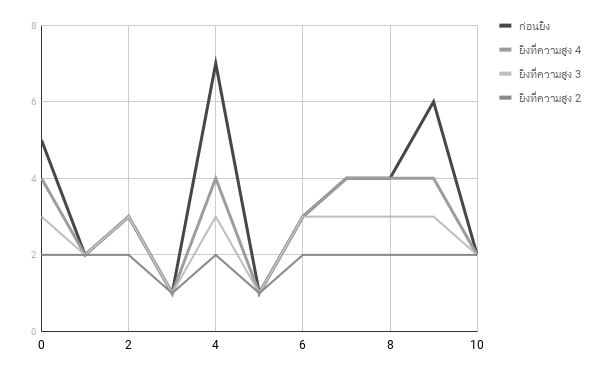
\includegraphics[width=\textwidth]{chart.png}

\end{problem}

\pagebreak
%%%%%%%%%%%%%%%%%%%%%%%%%%%%%%%%%%%%%%%%%%%%%%%%%%%%%%%%%%%%%%%%%%%%%%%%%%%%%%%%%%%%%%%%%%%

\begin{problem}{สมบัติล้ำค่า}{standard input}{standard output}{1 seconds}{256 megabytes}{100}

บริษัทแห่งหนึ่งได้ทำการส่งสินค้าชิ้นหนึ่งผ่านทางรถไฟ โดยสินค้าชิ้นนั้นเป็นสมบัติที่ขุดพบภายในโบราณสถานแห่งหนึ่ง เพื่อนำไปค้นคว้าหาข้อมูลต่อไป

กลุ่มบุคคลกลุ่มหนึ่งได้รู้ถึงข้อมูลเหล่านี้จึงได้ขึ้นรถไฟเพื่อพยายามที่จะขโมยสมบัติ จนได้พบสมบัติที่ตามหา แต่ปัญหามีกระจกครอบสมบัติไว้จำนวน $t$ ชั้น มีแป้นกดตัวเลข $0-9$ และได้มีข้อความเขียนไว้ว่า 

"ถ้าอยากจะได้สมบัติไป จงแก้ปัญหาต่อไปนี้ มีแผ่นกระเบื้องสีขาวและสีดำขนาด $1*1$ อยู่ไม่จำกัดแผ่น ต้องการวางแผ่นกระเบื้องให้เป็นทางยาวขนาด $2*n$ โดยที่กระเบื้องสีดำห้ามวางอยู่ติดกันเด็ดขาด จะสามารถวางได้ทั้งหมดกี่วิธีที่แตกต่างกัน โดยให้ตอบเป็นเศษที่เกิดจากการหารคำตอบด้วย $98765431$"

เมื่อพวกเขาได้อ่านเลยคิดว่าคงเป็นไปไม่ได้ เพราะไม่รู้ $n$ เลยพยายามจะทำลายกระจก แต่มันก็ทนทานจนเกินไป จนได้สังเกตว่ารอบๆ โบกี้ที่บรรทุกสมบัติมีตัวเลขที่เป็นค่าของ $n$ ถูกเขียนเป็นจำนวน $t$ ค่า เลยรู้ได้ทันทีว่าต้องตอบทั้งหมด $t$ ครั้งกระจกจึงจะเปิดหมด เลยอยากให้คุณซึ่งเป็นโปรแกรมเมอร์คนเดียวในทีมแก้ปัญหานี้ เพื่อสมบัติที่อาจเป็นของล้ำค่าได้

\InputFile
บรรทัดที่ $1$ รับจำนวนเต็ม $t$ แสดงถึงจำนวนคำถาม $(1 \leq t \leq 10^3)$

บรรทัดที่ $2$ ถึง $t + 1$ รับจำนวนเต็ม $n_i$ $(1 \leq n_i \leq10^{18})$
\OutputFile
มีจำนวน $t$ บรรทัด ซึ่งบรรทัดที่ $i$ แสดงคำตอบของคำถามที่ $i$ 
\Scoring
ชุดทดสอบจะถูกแบ่งเป็น $3$ ชุด จะได้คะแนนในแต่ละชุดก็ต่อเมื่อโปรแกรมให้ผลลัพธ์ถูกต้องในชุดทดสอบย่อยทั้งหมด

\begin{description}

\item[ชุดที่ 1 (10 คะแนน)]  $1 \leq t \leq 15 , 1 \leq n_i \leq 15$ 

\item[ชุดที่ 2 (25 คะแนน)] $1 \leq t \leq 100 , 1 \leq n_i \leq 10^{6}$

\item[ชุดที่ 3 (65 คะแนน)] ไม่มีเงื่อนไขเพิ่มเติม

\end{description}

\Examples

\begin{example}
\exmp{3
1
2
4
}{3
7
41
}%
\exmp{7
12
15
14
4
3
14
5
}{47321
665857
275807
41
17
275807
99
}%
\end{example}

\Note
\begin{note}
ยกตัวอย่างกรณีที่ $n = 2$ สามารถวางได้ 7 แบบที่แตกต่างกันดังนี้

\begin{center}
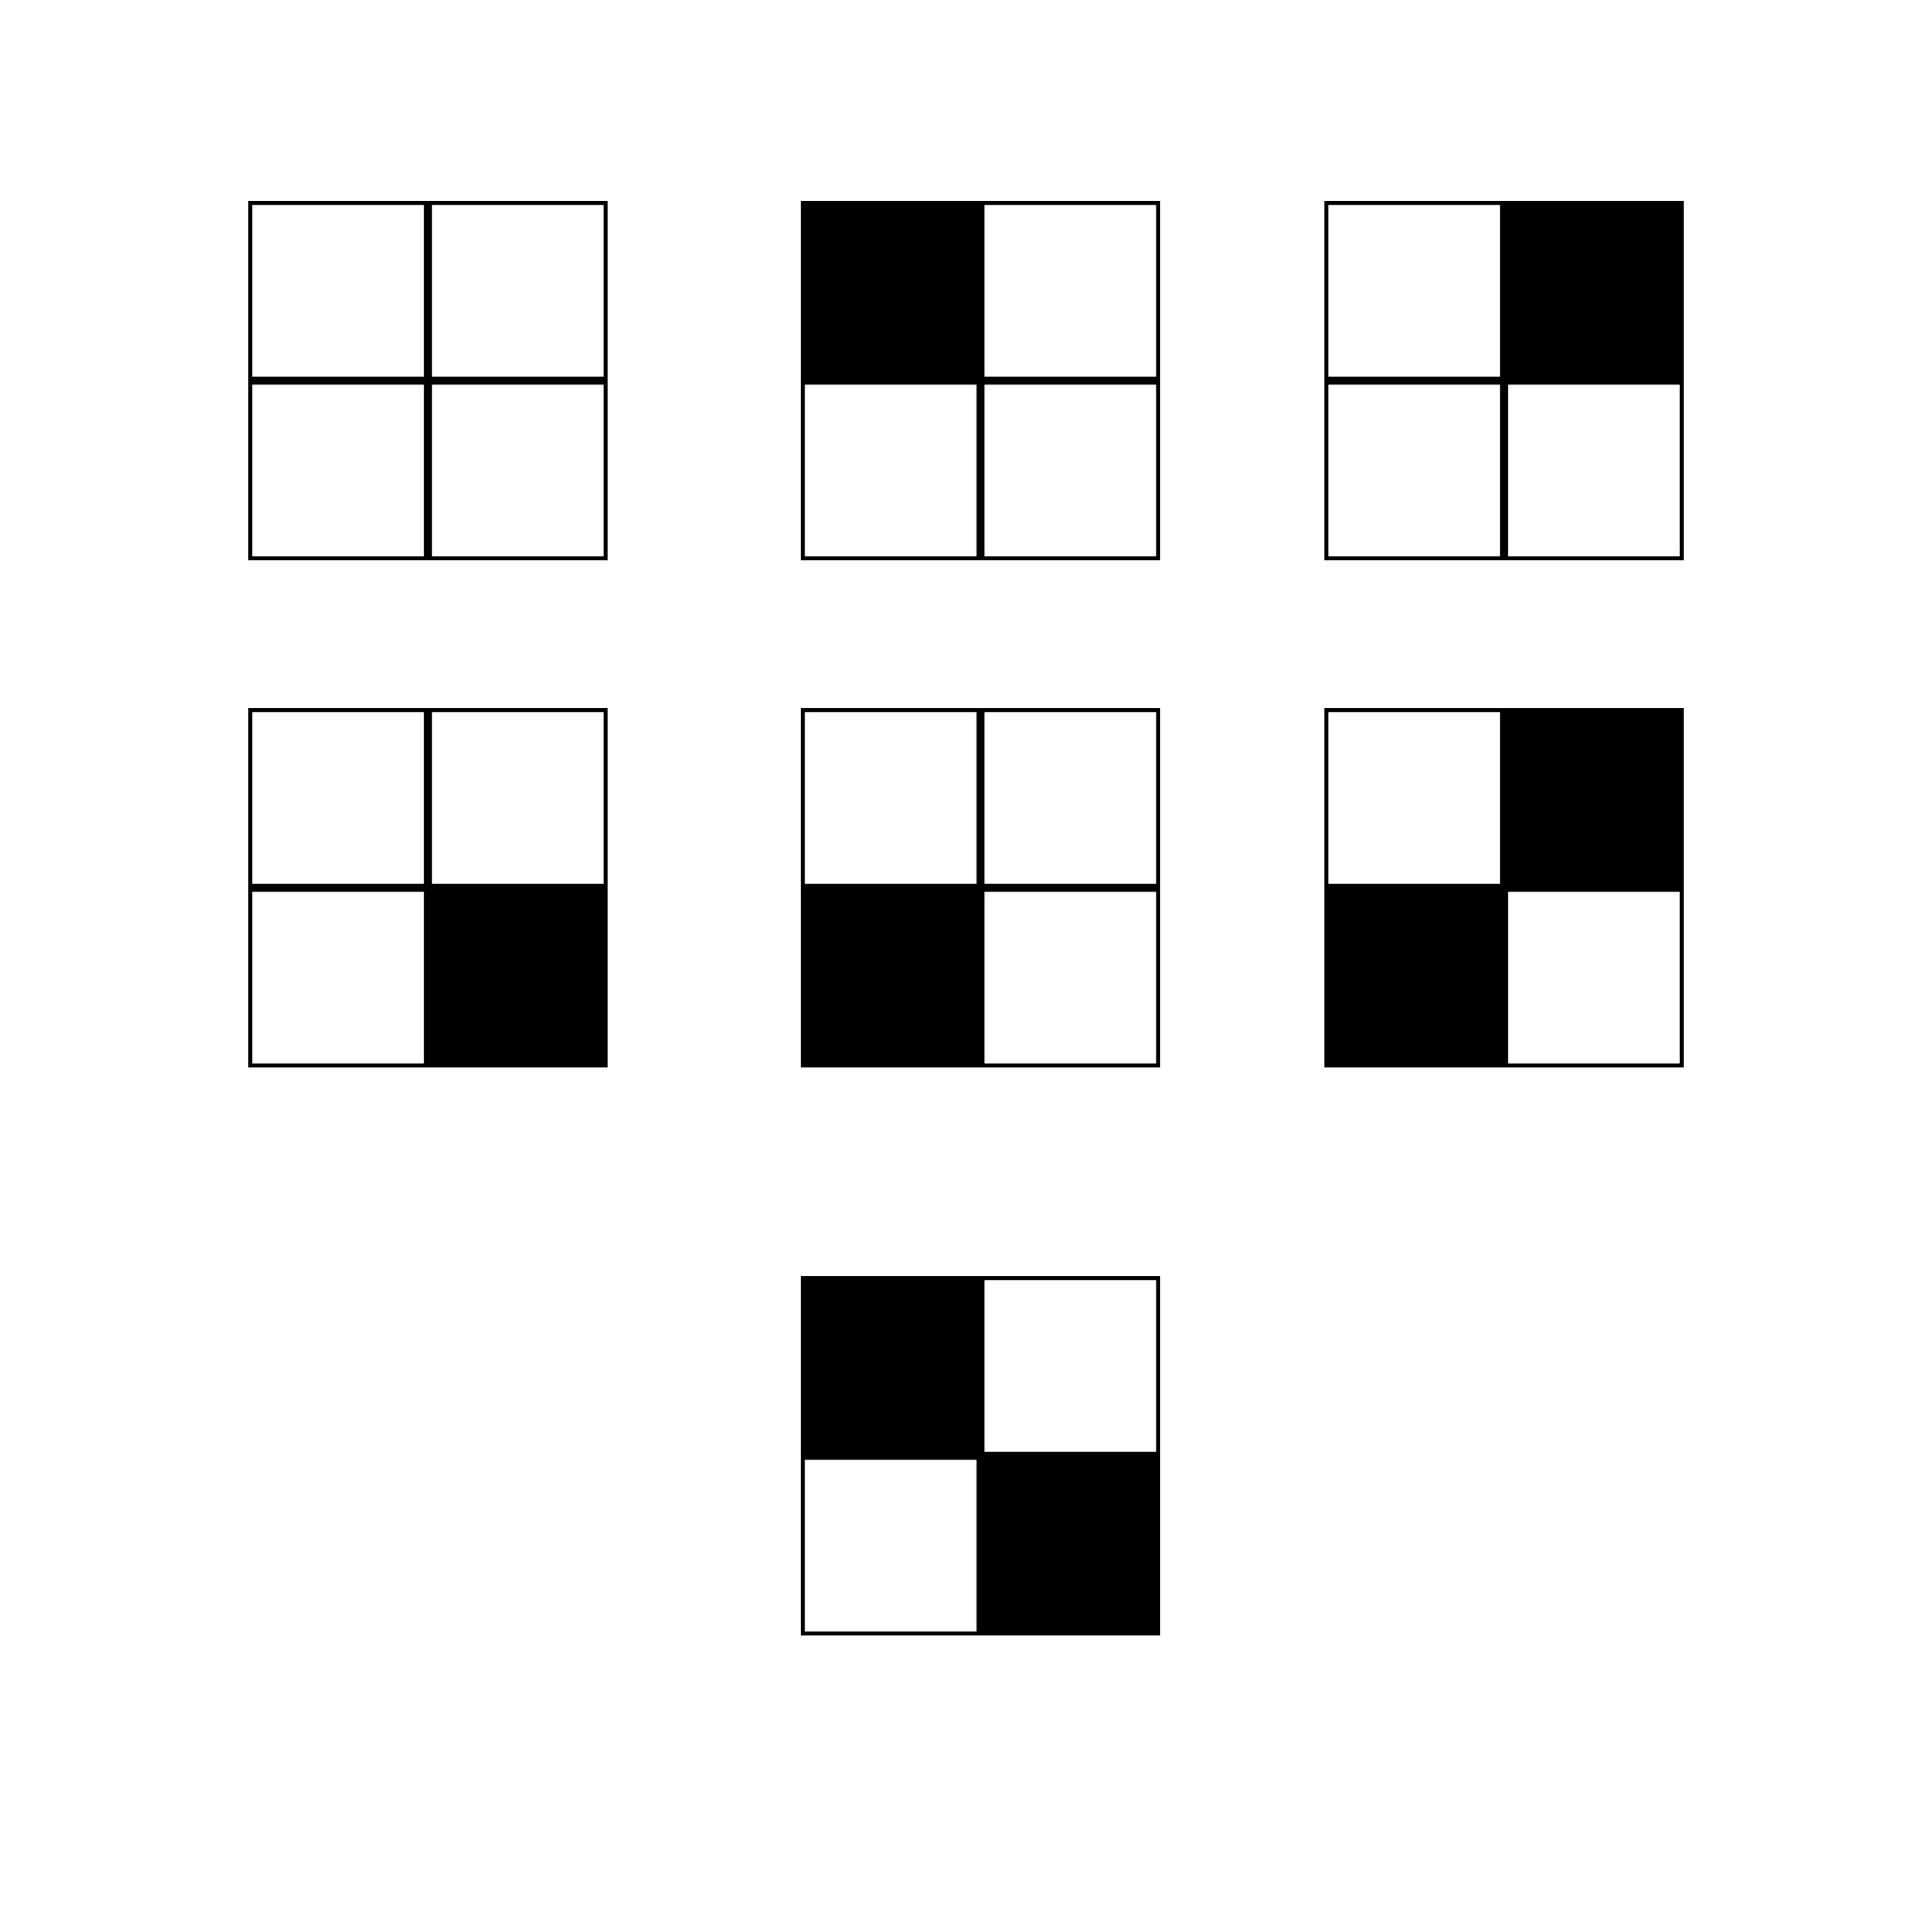
\includegraphics[width=8cm]{Sample.jpg}
\end{center}

\end{note}

\end{problem}

\pagebreak
%%%%%%%%%%%%%%%%%%%%%%%%%%%%%%%%%%%%%%%%%%%%%%%%%%%%%%%%%%%%%%%%%%%%%%%%%%%%%%%%%%%%%%%%%%%

\begin{problem}{Autocomplete}{standard input}{standard output}{1 second}{256 megabytes}{100}

  ภาษา TUMSO (The Untyped Microlanguage without Strings and Objects) เป็นภาษาที่ใช้สำหรับการคำนวณจำนวนเต็ม

  \subsection*{ภาษา TUMSO}

  ไวยากรณ์ของภาษา TUMSO มีดังนี้ (ให้อ่าน \texttt{::=}  ว่า "คือ" และอ่าน \texttt{|} ว่า "หรือ")

  \begin{codetumso}[frame=single]
<program> ::= <expression>

<expression> ::= <number>
               | TRUE
               | FALSE
               | <identifier>
               | (CALL <expression> <expression>)
               | (FUNCTION (<identifier>) <expression>)
               | (LET <identifier> = <expression> IN <expression>)
               | (IF <expression> THEN <expression> ELSE <expression>)
               | (PLUS <expression> <expression>)
               | (MINUS <expression> <expression>)
               | (IS_EQUAL <expression> <expression>)
  \end{codetumso}

  \begin{itemize}
    \item \texttt{<number>} เป็นจำนวนเต็ม ตัวอย่างเช่น \texttt{-1234}
    \item \texttt{<identifier>} เป็นชื่อตัวแปร ประกอบไปด้วยอักขระในช่วง \texttt{a} ถึง \texttt{z} และเครื่องหมาย \texttt{\_} เช่น \texttt{the\_sum\_of\_two\_numbers}
  \end{itemize}

  โทเคนในภาษานี้ได้แก่ ตัวเลข \texttt{TRUE} \texttt{FALSE} \texttt{CALL} \texttt{FUNCTION} \texttt{LET} \texttt{=} \texttt{IN} \texttt{IF} \texttt{THEN} \texttt{ELSE} \texttt{PLUS} \texttt{MINUS} \texttt{IS\_EQUAL} และตัวแปร โดยโทเคนจะต้องถูกแยกออกจากกันด้วยช่องว่าง วงเล็บ หรืออักขระขึ้นบรรทัด

  \pagebreak

  \subsection*{ความหมายของโครงสร้างทางภาษา}

  \begin{itemize}
    \item สำหรับตัวเลข และ \texttt{TRUE} กับ \texttt{FALSE} จะได้ค่าผลลัพธ์เป็นเป็นค่าตัวเลข ค่า \texttt{TRUE} หรือค่า \texttt{FALSE} นั้น ๆ
    \item สำหรับตัวแปร จะได้ค่าผลลัพธ์เป็นค่าที่ตัวแปรนั้นเก็บอยู่
    \item สำหรับ \texttt{(CALL <f> <a>)} ค่าผลลัพธ์ของ \texttt{<f>} ควรจะเป็นค่าฟังก์ชัน และจะได้ค่าผลลัพธ์เป็นค่าของการเรียกใช้ฟังก์ชันนั้นด้วยพารามิเตอร์ซึ่งก็คือค่าผลลัพธ์ของ \texttt{<a>}
    \item สำหรับ \texttt{(FUNCTION (<a>) <e>)} จะได้ค่าผลลัพธ์เป็นค่าฟังก์ชันนั้น ๆ ที่มีพารามิเตอร์คือ \texttt{<a>} และเมื่อมีการเรียกฟังก์ชันด้วยพารามิเตอร์ \texttt{<v>} จะสร้างตัวแปร \texttt{<a>} ขึ้นมาเก็บค่า \texttt{<v>} และได้ค่าผลลัพธ์เป็น \texttt{<e>} (โดยที่ \texttt{<a>} สามารถถูกอ้างถึงได้ใน \texttt{<e>})
    \item สำหรับ \texttt{(LET <x> = <v> IN <e>)} จะสร้างตัวแปร \texttt{<x>} ขึ้นมาเก็บค่าของ \texttt{<v>} และได้ค่าผลลัพธ์เป็น \texttt{<e>} (โดยที่ \texttt{<x>} สามารถถูกอ้างถึงได้ในทั้ง \texttt{<v>} และ \texttt{<e>})
    \item สำหรับ \texttt{(IF <cond> THEN <then> ELSE <else>)} หาก \texttt{<cond>} มีค่าคือผลลัพธ์คือ \texttt{TRUE} จะได้ค่าผลลัพธ์เป็น \texttt{<then>} แต่หาก \texttt{<cond>} มีค่าคือผลลัพธ์คือ \texttt{FALSE} จะได้ค่าผลลัพธ์เป็น \texttt{<else>}
    \item สำหรับ \texttt{(PLUS <a> <b>)} ค่าผลลัพธ์ของ \texttt{<a>} และ \texttt{<b>} ควรจะเป็นตัวเลข และจะได้ค่าผลลัพธ์เป็น \texttt{<a>}~$+$~\texttt{<b>}
    \item สำหรับ \texttt{(MINUS <a> <b>)} ค่าผลลัพธ์ของ \texttt{<a>} และ \texttt{<b>} ควรจะเป็นตัวเลข และจะได้ค่าผลลัพธ์เป็น \texttt{<a>}~$−$~\texttt{<b>}
    \item สำหรับ \texttt{(IS\_EQUAL <a> <b>)} ค่าผลลัพธ์ของ \texttt{<a>} และ \texttt{<b>} ควรจะเป็นตัวเลข และจะได้ค่าผลลัพธ์เป็น \texttt{TRUE} หาก \texttt{<a>}~$=$~\texttt{<b>} และจะได้ค่าผลลัพธ์เป็น \texttt{FALSE} หาก \texttt{<a>}~$\ne$~\texttt{<b>}
  \end{itemize}

  \subsection*{ตัวอย่างโปรแกรมในภาษา TUMSO}

  \begin{tabular}{|M{12cm}|M{3.5cm}|N}
    \hline
    \textbf{โปรแกรม} & \textbf{ผลลัพธ์} & \\[5pt]
    \hline \hline

%%%%%%%%%%%%%%%%%%%%%%%%%%%%%%%%%%%%%%%%%%%%%%%%%%%%%%%%%%%%%%%%%%%%%%%%%%%%%%%%

    {\begin{codetumso}
FALSE
    \end{codetumso}} & {\begin{codetumso}
FALSE
    \end{codetumso}}
    \\ \hline

%%%%%%%%%%%%%%%%%%%%%%%%%%%%%%%%%%%%%%%%%%%%%%%%%%%%%%%%%%%%%%%%%%%%%%%%%%%%%%%%

    {\begin{codetumso}
(LET a = 1 IN
  (PLUS
    (LET a = 2 IN a)
    a))
    \end{codetumso}} & {\begin{codetumso}
3
    \end{codetumso}}
    \\ \hline

%%%%%%%%%%%%%%%%%%%%%%%%%%%%%%%%%%%%%%%%%%%%%%%%%%%%%%%%%%%%%%%%%%%%%%%%%%%%%%%%

    {\begin{codetumso}
(LET mult = (FUNCTION (a)
              (FUNCTION (b)
                (IF (IS_EQUAL 0 a)
                 THEN 0
                 ELSE (PLUS b (CALL (CALL mult b)
                                    (MINUS a 1)))))) IN
  (LET fact = (FUNCTION (n)
                (IF (IS_EQUAL 0 n)
                 THEN 1
                 ELSE (CALL (CALL mult n)
                            (CALL fact
                                  (MINUS n 1))))) IN
    (CALL fact 5)))
    \end{codetumso}} & {\begin{codetumso}
120
    \end{codetumso}}
    \\ \hline

%%%%%%%%%%%%%%%%%%%%%%%%%%%%%%%%%%%%%%%%%%%%%%%%%%%%%%%%%%%%%%%%%%%%%%%%%%%%%%%%

    {\begin{codetumso}
a
    \end{codetumso}} & {\begin{codetumso}
Error: `a' is undefined
    \end{codetumso}}
    \\ \hline

%%%%%%%%%%%%%%%%%%%%%%%%%%%%%%%%%%%%%%%%%%%%%%%%%%%%%%%%%%%%%%%%%%%%%%%%%%%%%%%%

    {\begin{codetumso}
(CALL 1 2)
    \end{codetumso}} & {\begin{codetumso}
Error: type mismatch
    \end{codetumso}}
    \\ \hline

  \end{tabular}

\section*{Task}

  ปัญหาการเรียกใช้ตัวแปรที่ไม่ได้ถูกนิยามไว้เป็นปัญหาที่พบได้ในภาษาโปรแกรมส่วนใหญ่ รวมถึงภาษา TUMSO ด้วย (ดูตัวอย่างโปรแกรมที่ 4 เป็นต้น) บาง IDE (Integrated development environment) เช่น Eclipse ของภาษา Java มีเครื่องมือแนะนำ\textit{ตัวแปรที่สามารถใช้ได้} ในตำแหน่งที่เคอร์เซอร์กำลังอยู่ เพื่อที่คุณจะได้ไม่เขียนโปรแกรมผิดตั้งแต่แรก

  \begin{figure}[h]
    \centering
    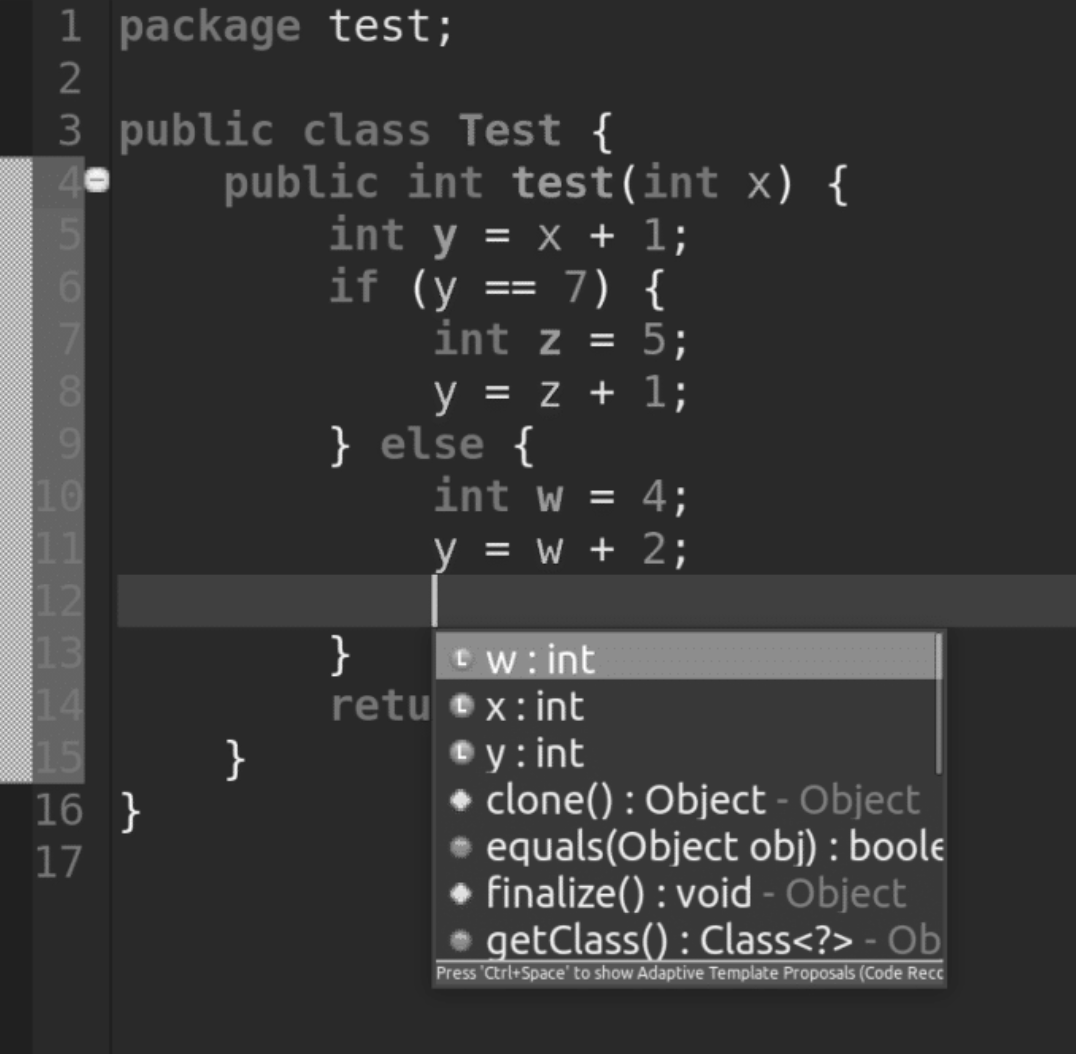
\includegraphics[width=0.6\textwidth]{calc-vars}
    \caption{ตัวอย่างโปรแกรม Eclipse ที่แนะนำตัวแปรที่สามารถใช้งานได้ในตำแหน่งที่เคอร์เซอร์อยู่สำหรับภาษา Java }
  \end{figure}

  หน้าที่ของคุณคือให้เขียนโปรแกรมรับโค้ดที่ไม่สมบูรณ์ในภาษา TUMSO โดยมีสัญลักษณ์ \texttt{\#} อยู่หนึ่งที่ในตำแหน่ง \texttt{<expression>} (แสดงถึงเคอร์เซอร์ในโปรแกรมที่กำลังเขียนอยู่) และแสดงผลตัวแปรทั้งหมดที่สามารถใช้ได้ที่ตำแหน่ง \texttt{\#}

\InputFile

  ประกอบไปด้วยโค้ดที่ไม่สมบูรณ์ในภาษา TUMSO ซึ่งมีอักขระ \texttt{\#} อยู่หนึ่งที่ในตำแหน่ง \texttt{<expression>} และหากแทนที่อักขระ \texttt{\#} ในโค้ดนี้ด้วย \texttt{<expression>} ใด ๆ (เช่น \texttt{0}) จะทำให้กลายเป็นโปรแกรมที่มีไวยากรณ์ถูกต้องในภาษา TUMSO โค้ดนี้จะมีความยาวกี่บรรทัดก็ได้

\OutputFile

  มี $n$ บรรทัด โดย $n$ คือจำนวนตัวแปรที่สามารถใช้ได้ในตำแหน่ง \texttt{\#} และแต่ละบรรทัดมีชื่อของตัวแปรที่สามารถใช้ได้ดังกล่าวในลำดับพจนานุกรม (lexicographic order)

\section*{Constraints}

  โค้ดที่ให้จะมีขนาดไม่เกิน $10^6$ ไบต์

\Examples

  \begin{tabular}{|M{12cm}|M{3.5cm}|N}
    \hline
    \textbf{ข้อมูลนำเข้า} & \textbf{ข้อมูลส่งออก} & \\[5pt]
    \hline \hline

%%%%%%%%%%%%%%%%%%%%%%%%%%%%%%%%%%%%%%%%%%%%%%%%%%%%%%%%%%%%%%%%%%%%%%%%%%%%%%%%

    {\begin{codetumso}
(LET mult = (FUNCTION (a)
              (FUNCTION (b)
                (IF (IS_EQUAL 0 a)
                 THEN 0
                 ELSE (PLUS b (CALL (CALL mult b)
                                    (MINUS a 1)))))) IN
  (LET fact = (FUNCTION (n)
                (IF (IS_EQUAL 0 n)
                 THEN 1
                 ELSE (CALL (CALL mult n)
                            (CALL fact
                                  (MINUS n 1))))) IN
    (CALL fact #)))
    \end{codetumso}} & {\begin{codetumso}
fact
mult
    \end{codetumso}}
    \\ \hline

%%%%%%%%%%%%%%%%%%%%%%%%%%%%%%%%%%%%%%%%%%%%%%%%%%%%%%%%%%%%%%%%%%%%%%%%%%%%%%%%

    {\begin{codetumso}
(IF TRUE THEN a ELSE (LET x = 1 IN #))
    \end{codetumso}} & {\begin{codetumso}
x
    \end{codetumso}} \\ \hline
\end{tabular}

\end{problem}



\end{document}
